\documentclass[10pt, compress]{beamer}
\usetheme[titleprogressbar]{m}

\usepackage{booktabs}
\usepackage[scale=2]{ccicons}
\usepackage{minted}

\usepackage{caption}
\captionsetup[figure]{labelformat=empty}
\captionsetup{skip=0pt, belowskip=0pt}

\usepgfplotslibrary{dateplot}

\usemintedstyle{trac}

\title{Poisson Processes and 911 Calls}
\subtitle{}
\date{\today}
\author{Jacob Mortensen}
\institute{Brigham Young University}

\begin{document}
  \maketitle
  
  \section{Introduction}
  \begin{frame}
    \frametitle{Introduction}
    \begin{itemize}
      \item Extreme heat scenarios pose a significant threat to public health
      \item It is of interest for researchers to understand how the effect of heat varies by location
    \end{itemize}
  \end{frame}
  \begin{frame}
    \frametitle{Introduction}
    \centering
    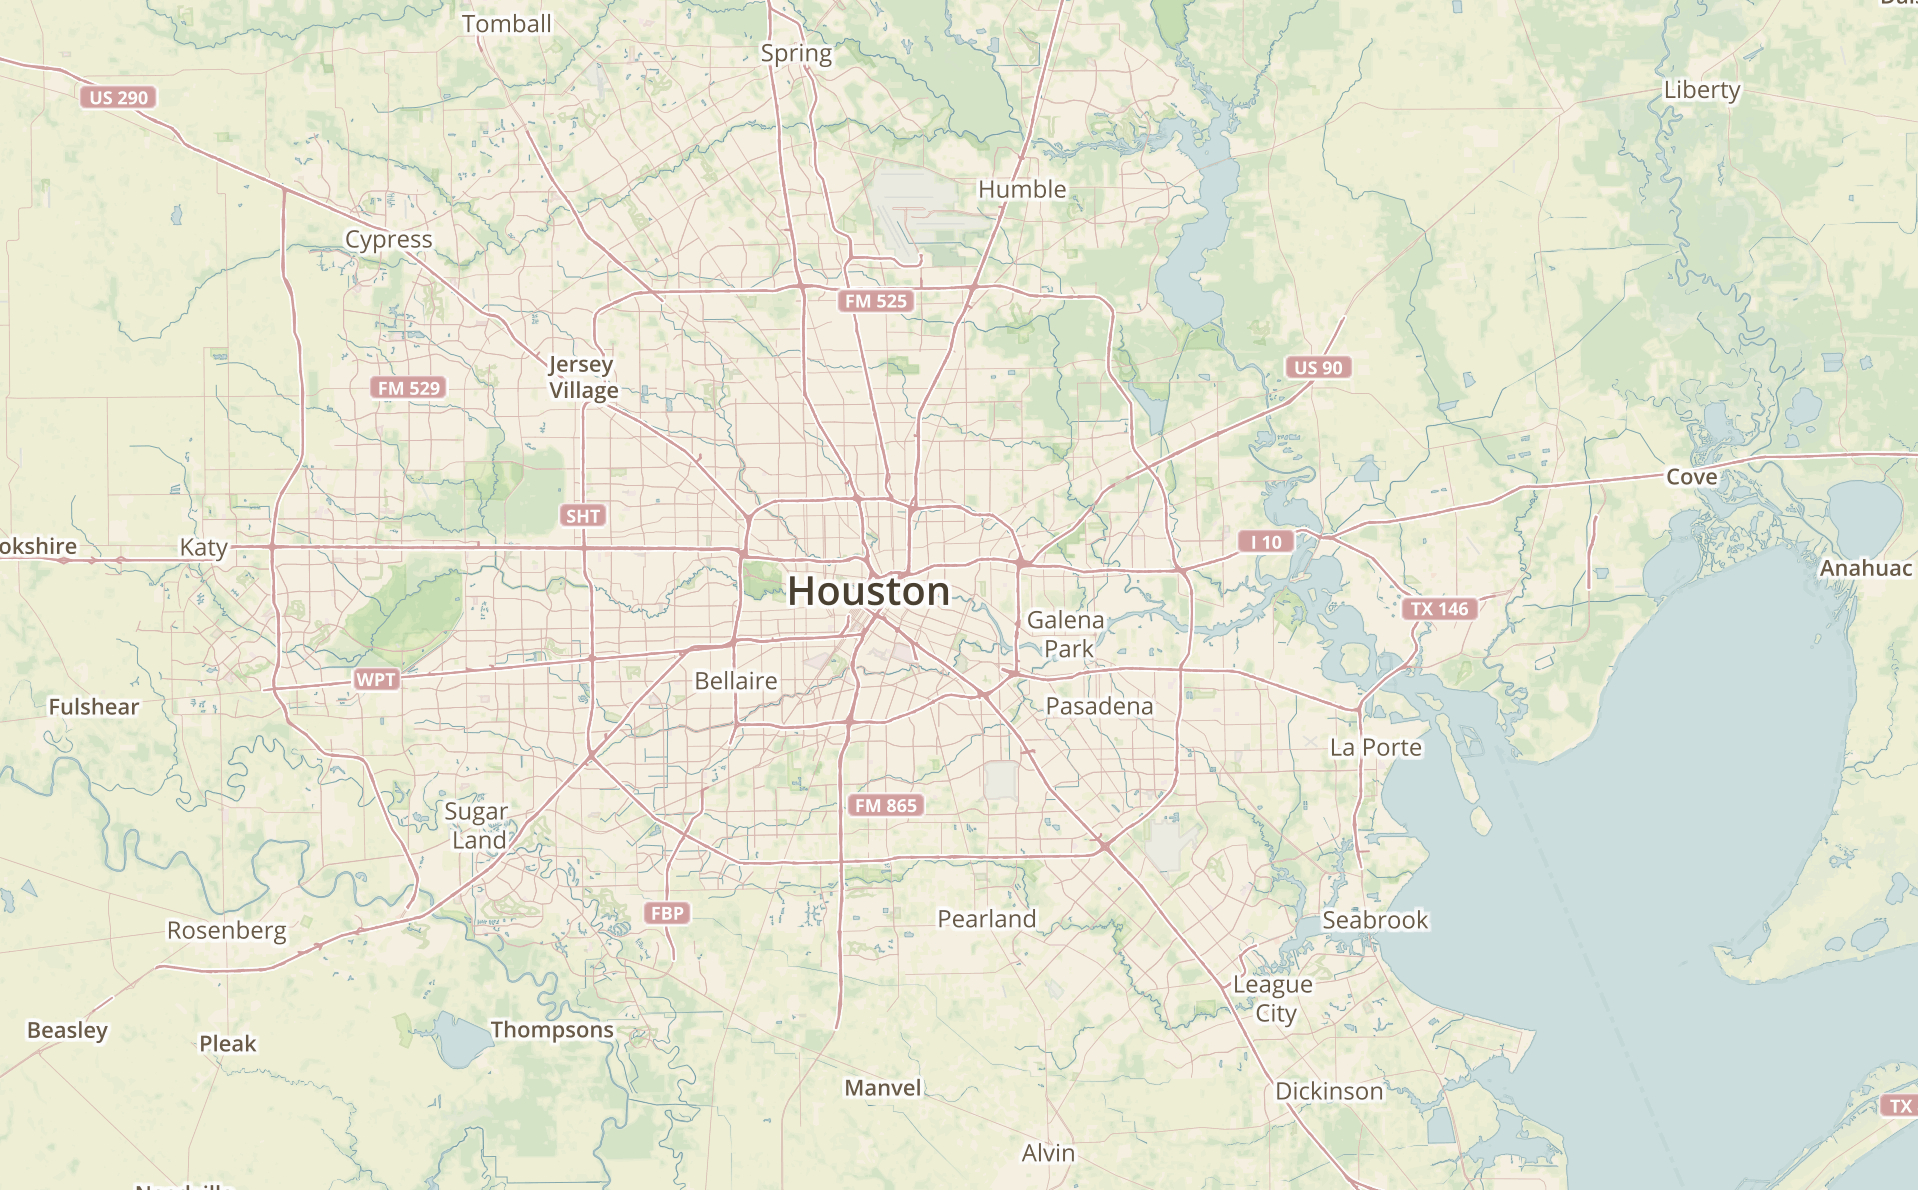
\includegraphics[width=0.8\textwidth]{houston_map.jpg}
  \end{frame}
  \begin{frame}{Introduction}
    \centering
    \begin{minipage}{0.8\textwidth}
      Spatial data is:
      \begin{itemize}
        \item nonlinear
        \item highly correlated
      \end{itemize}
    so how do we model it?
    \end{minipage}
  \end{frame}
  \section{Point Processes}
  \begin{frame}
    \frametitle{Point Process Models}
     
    Say something about the intensity surface here
  \end{frame}

  \section{Model}
  \begin{frame}
    \frametitle{Model}
      \begin{itemize}
        \item $N \sim Pois(\int_{s\in \mathbf{S}} \Lambda(s))$
        \item $\mathbf{s}$ is a vector of N = 1389 observed 911 call locations
        \item $\mathbf{S}$ is the set of all possible spatial locations
        \item $L(\Lambda(s)) = e^{\int_{s\in\mathbf{S}}\Lambda(s)}\cdot \prod_{i=1}^{N}\Lambda(\mathbf{s}_i)$
      \end{itemize}
  \end{frame}
  \begin{frame}
    \frametitle{Model}
    \begin{itemize}
      \item $\mathbf{s}^{*}$ is K = 1428 spatial prediction locations
      \item We can discretize $\Lambda(s)$ to make modeling easier:
    \end{itemize}
        $$ \Lambda(s) = \delta \sum_{k=1}^K \lambda_k 1 \left\{ \mathbf{s} \in \mathcal{G}_k \right\} $$
  \end{frame}
  \begin{frame}
    \frametitle{Model}
    \centering
    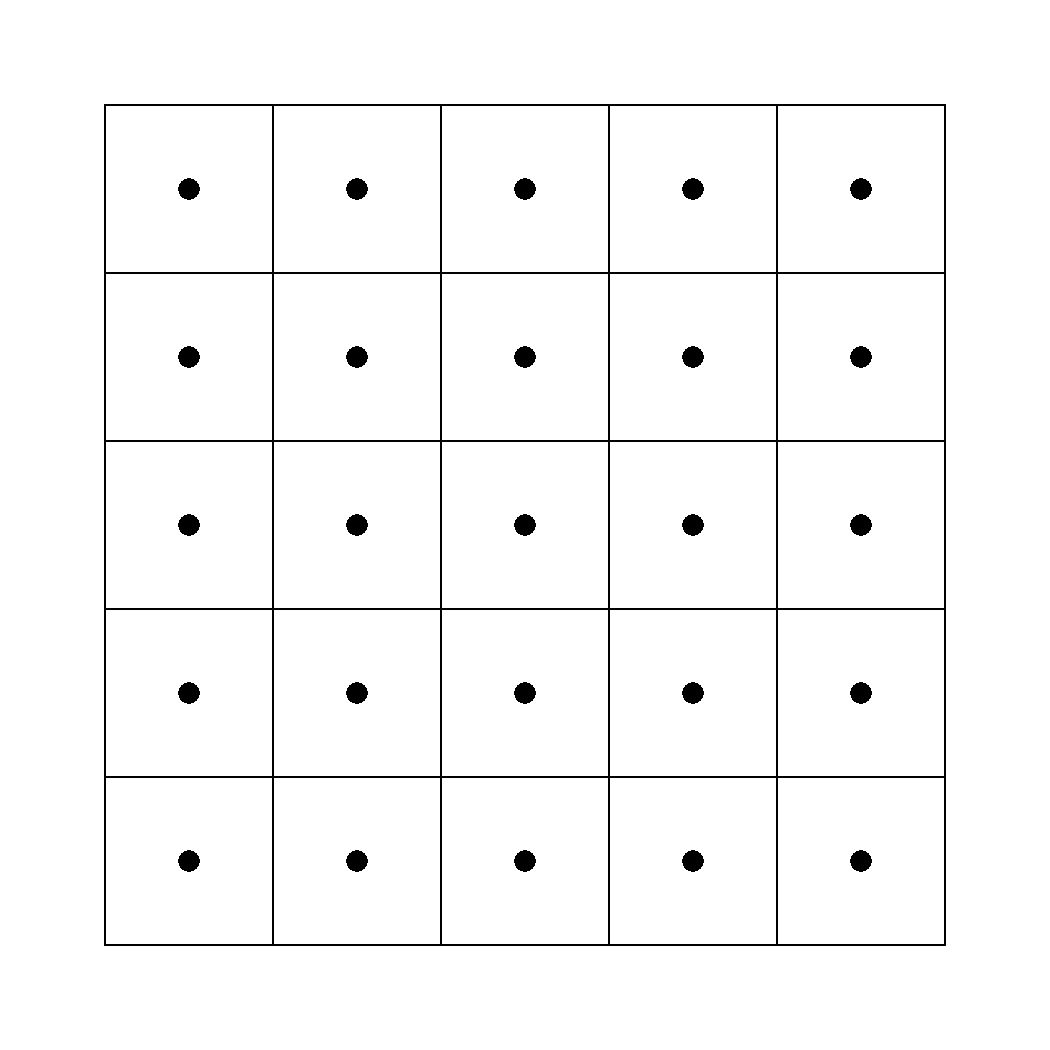
\includegraphics[height=0.8\textheight]{blank_grid.pdf}
  \end{frame}
  \begin{frame}
    \frametitle{Model}
    \centering
    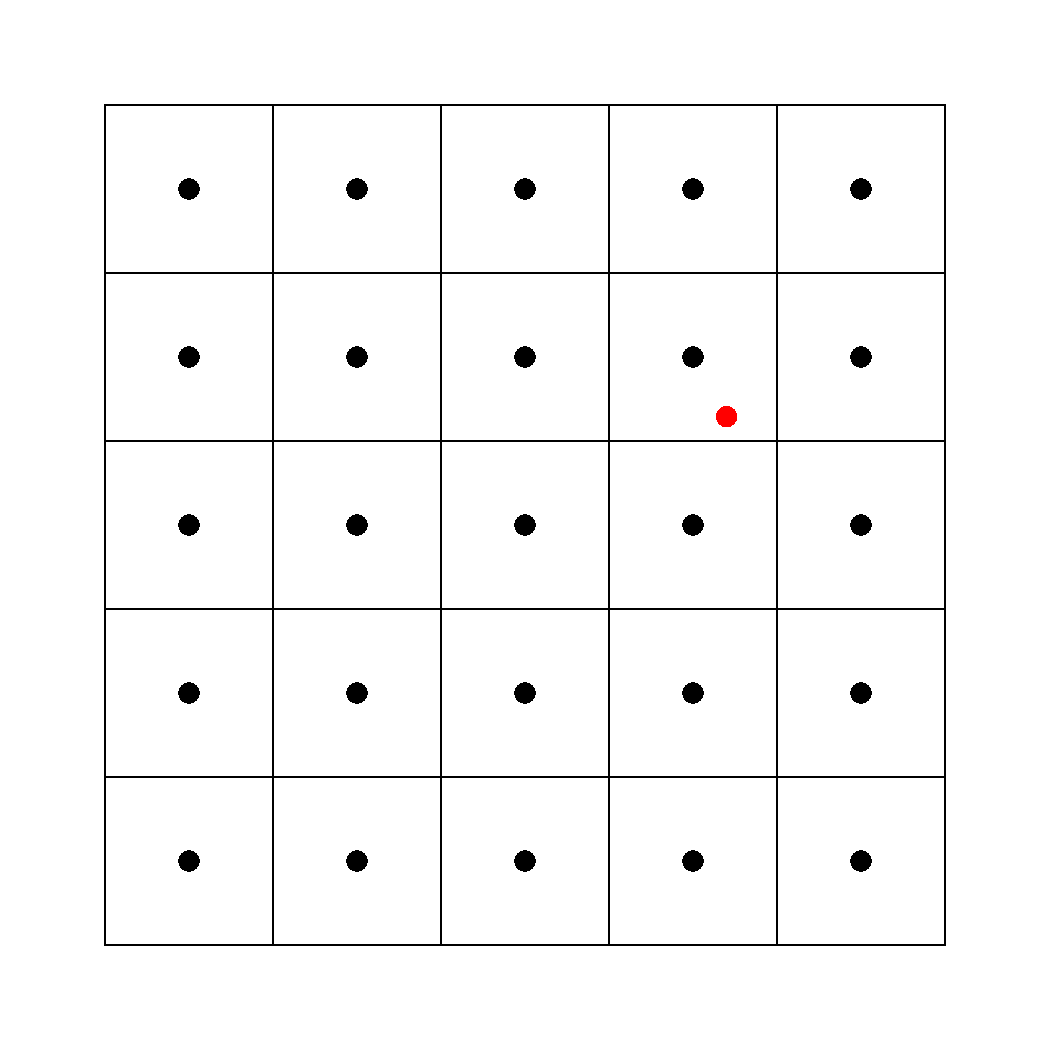
\includegraphics[height=0.8\textheight]{grid_spot.pdf}
  \end{frame}
  
\end{document}
